\section{Background Theory}

\subsection{Battery Safety}

Some of the obstacles of using Lithium batteries were the safety aspects involved as certain Lithium batteries can be volatile, catch fire or even explode.
\newline
The LiFe batteries were chosen for this very reason as they were reportedly robust and highly stable, which meant that they were reasonably safe to use on Tiberius III with proper protection.

\subsection{Star Grounding}
In light of optimising circuits and wiring, we tried to adopt star grounding wherever possible.  This meant putting every component's ground into one common ground, known as the star ground point, so that all conductors extend outwards to form a 'star'. This was implemented for all of the high power devices as shown in Figure \ref{fig:Cabling}.

\begin{figure}[!htb]
\begin{center}
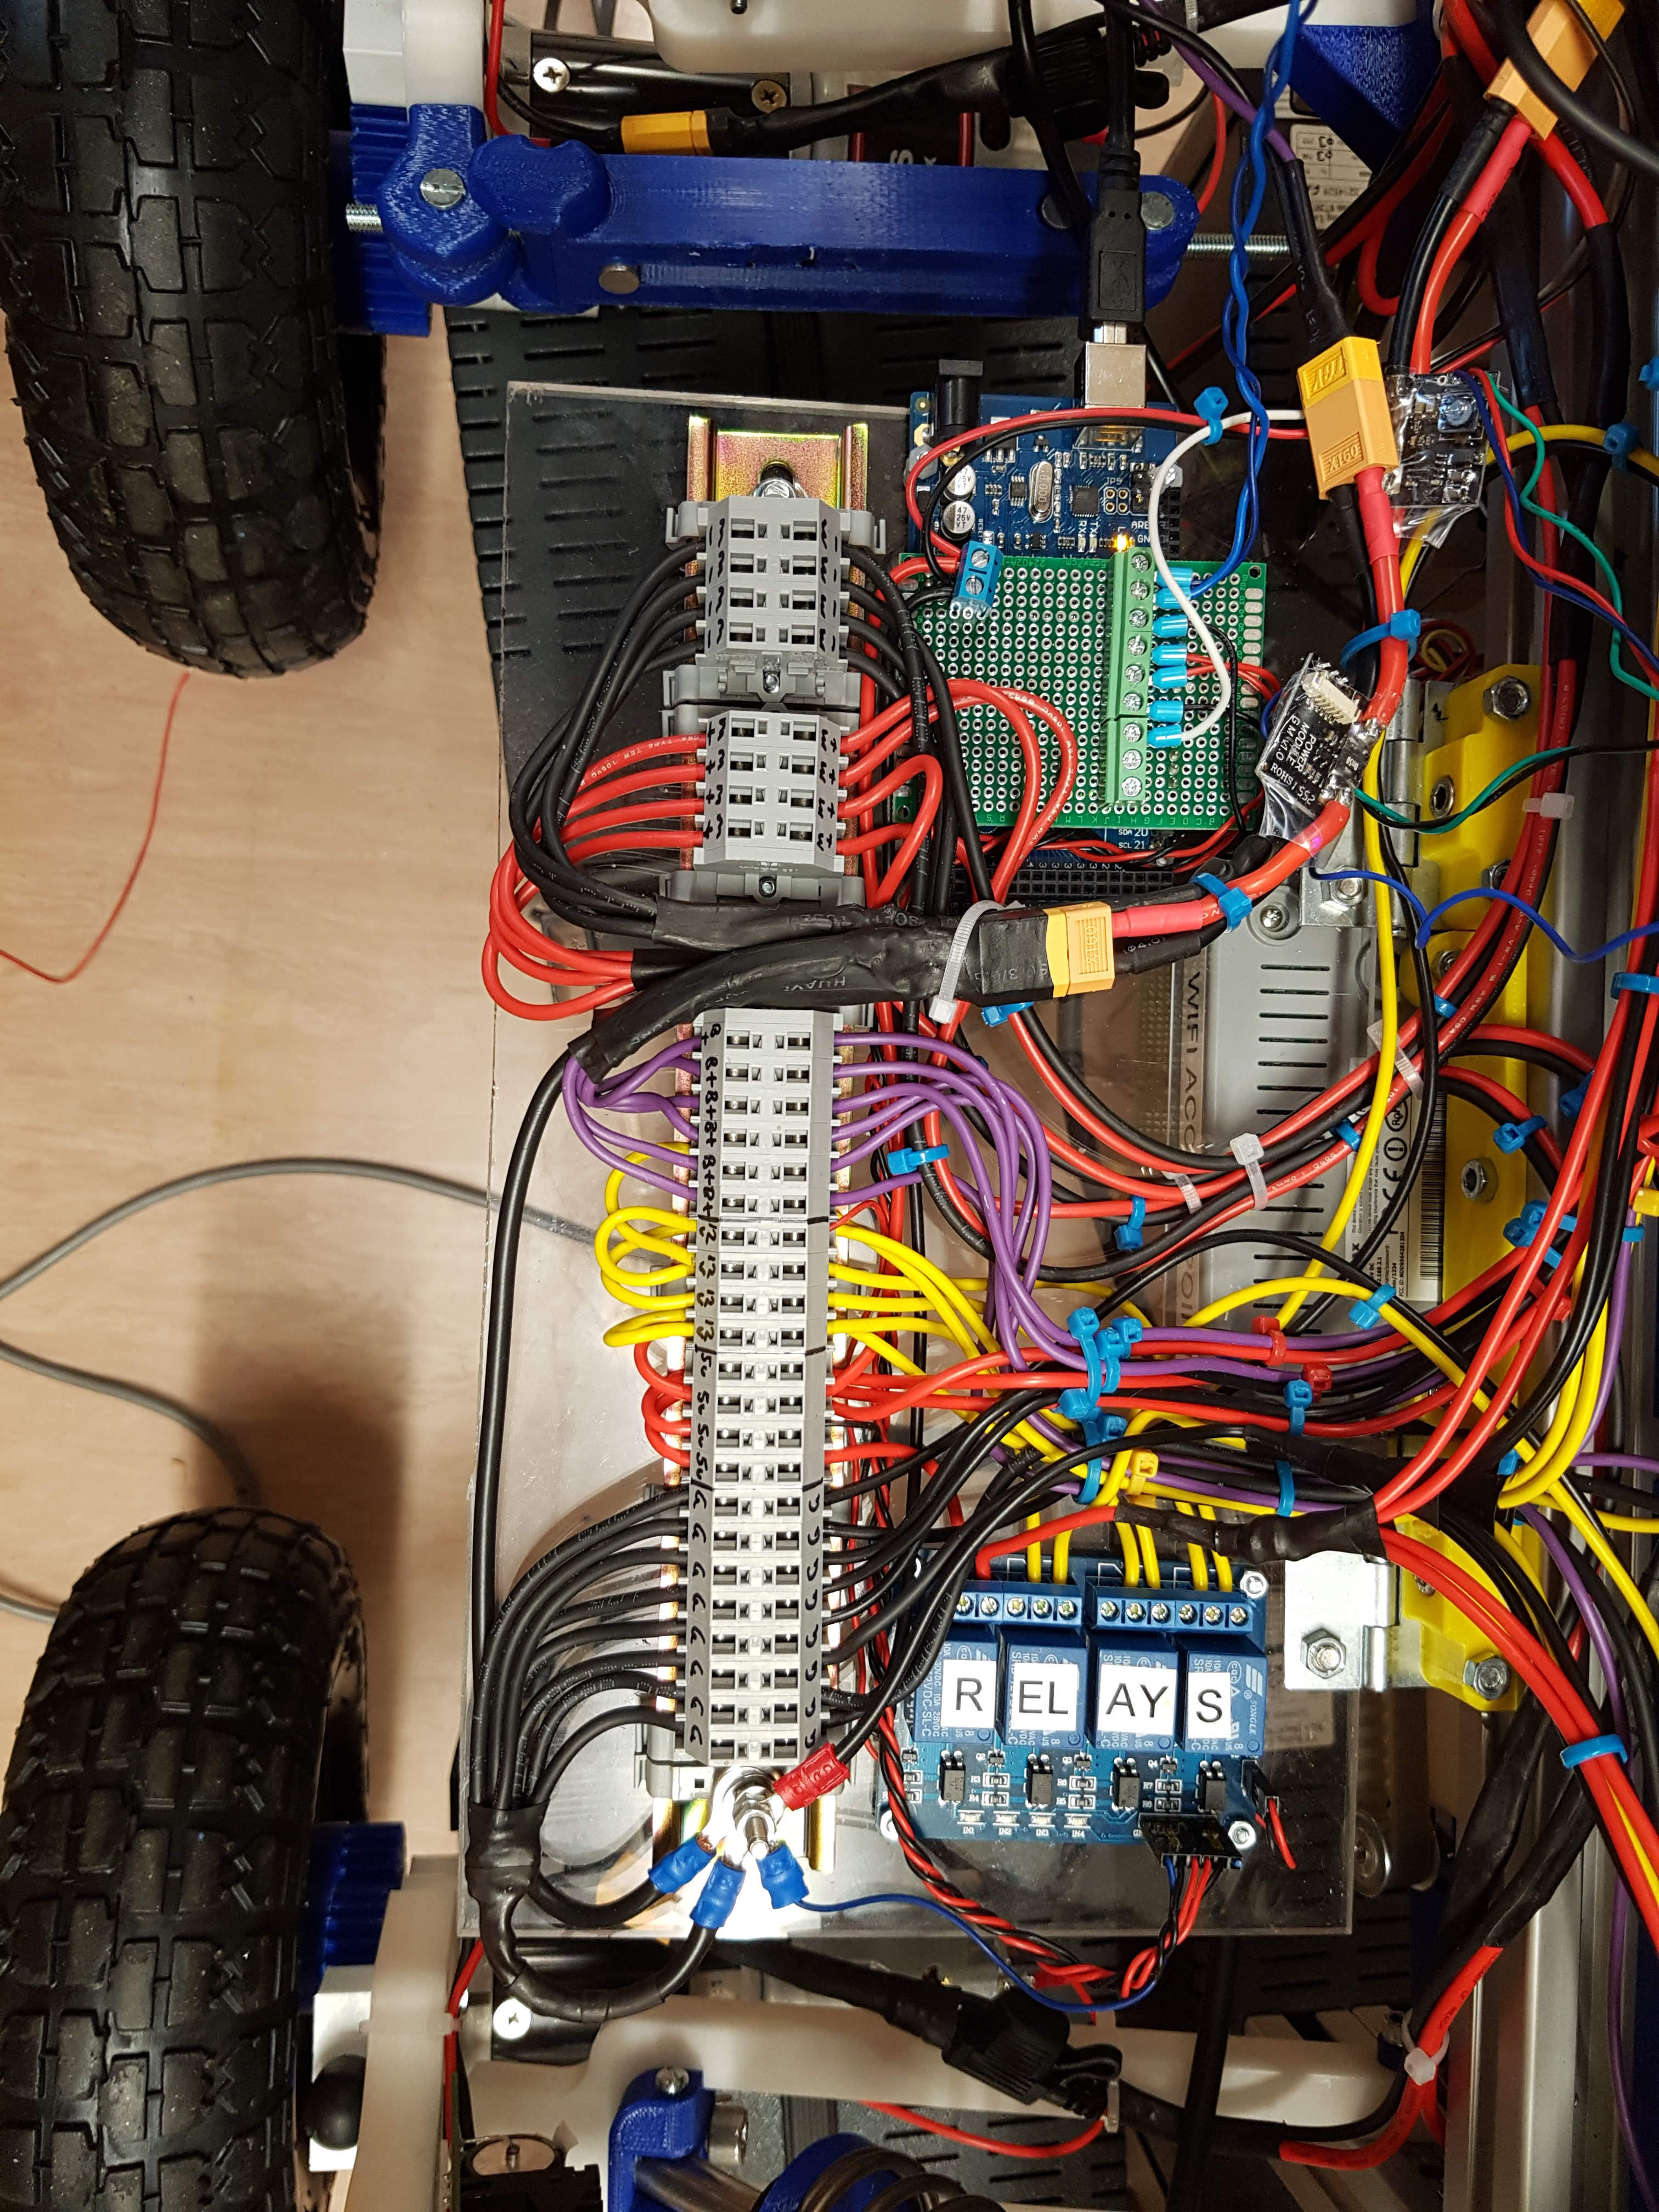
\includegraphics[width=6cm]{cabling.jpg}
\end{center}
\caption{Star Grounding}
\label{fig:Cabling}
\end{figure}